
\begin{esimerkki}
        Murtolukujen yhteenlasku. Laske
        \[
        \frac{1}{2} + \frac{1}{6} + \frac{2}{6}.
        \]
        
        \textbf{Ratkaisu.}
        Lavennetaan nimittäjät samannimisiksi ja lasketaan osoittajat yhteen:
        %lisätäänkö lavennusmerkki? teknisesti hankala? käytetäänkö maailmalla? opiskelijoille kuitenkin tuttu
        %tai sitten voisi sanallisesti kertoa, millä lavennetaan.
        \begin{align*}
            \frac{1}{2} + \frac{1}{6} + \frac{2}{6} &=\frac{3\cdot 1}{3\cdot 2} + \frac{1}{6} + \frac{2}{6}\\
            										&=\frac{3}{6} + \frac{1}{6} + \frac{2}{6}\\
           											&= \frac{3+1+2}{6}\\
           											&= \frac{6}{6} = 1.
        \end{align*}
    \end{esimerkki}

\laatikko{
    Jos murtolukujen
    nimittäjät ovat samat, voidaan murtoluvut laskea yhteen laskemalla
    osoittajat yhteen.
    \[
    \frac{a}{c} + \frac{b}{c} = \frac{a+b}{c}
    \]
}

    Murtolukuja, joiden nimittäjät ovat samat, sanotaan \termi{samanniminen}{samannimisiksi}.
    Jos yhteenlaskettavien murtolukujen nimittäjät eivät ole samat, murtoluvut
    \termi{laventaminen}{lavennetaan} ensin samannimisiksi ja sitten osoittajat lasketaan yhteen.
    Jos siis $\frac{a}{b}$ ja $\frac{c}{d}$ ovat murtolukuja, lasketaan

\laatikko{
    \[
    \frac{a}{b} + \frac{c}{d} = \frac{ad}{bd} + \frac{bc}{bd} = \frac{ad+bc}{bd}
    \]
    Tässä $\frac{a}{b}$ lavennetaan luvulla $d$ ja $\frac{c}{d}$ lavennetaan
    luvulla $b$, jolloin saadaan kaksi samannimistä murtolukua, joiden kummankin
    nimittäjä on yhteenlaskettavien nimittäjien tulo $bd$.
 }    

\begin{esimerkki}
        Murtolukujen kertolaskussa osoittajat ja nimittäjät kerrotaan keskenään.
      \[
        \frac{3}{4}\cdot \frac{6}{5}= \frac{3\cdot 6}{4\cdot 5}= \frac{18}{20}=\frac{9}{10}
        \]
    \end{esimerkki}
\laatikko{
    Murtolukujen $\frac{a}{b}$ ja $\frac{c}{d}$ tulo lasketaan kertomalla lukujen osoittajat ja nimittäjät keskenään:
    % Onko tämä toistoa? sama sanottiin jo yllä olevassa esimerkissä.
    \[
    \frac{a}{b}\cdot \frac{c}{d} = \frac{a\cdot c}{b\cdot d} = \frac{ac}{bd}
    \]
}

%\missingfigure{tähän Sampon paperille suunnittelema havainnollistus kertolaskusäännöstä}
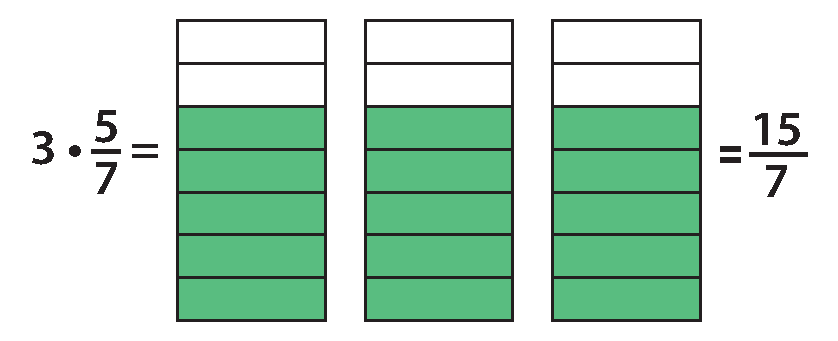
\includegraphics[scale=0.4]{pictures/Kuva3-1-1.pdf}
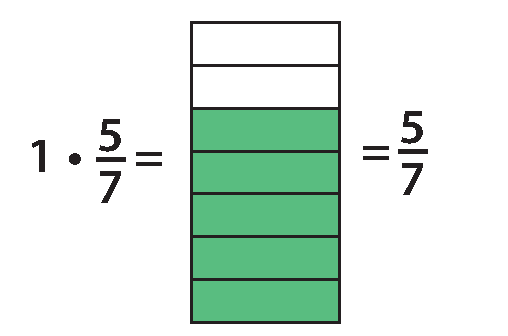
\includegraphics[scale=0.4]{pictures/Kuva3-1-2.pdf}
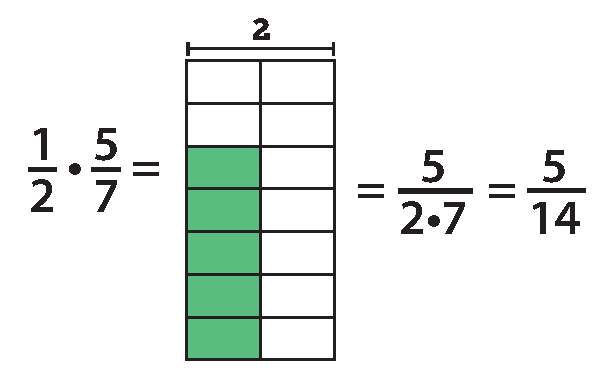
\includegraphics[scale=0.4]{pictures/Kuva3-1-3.pdf}
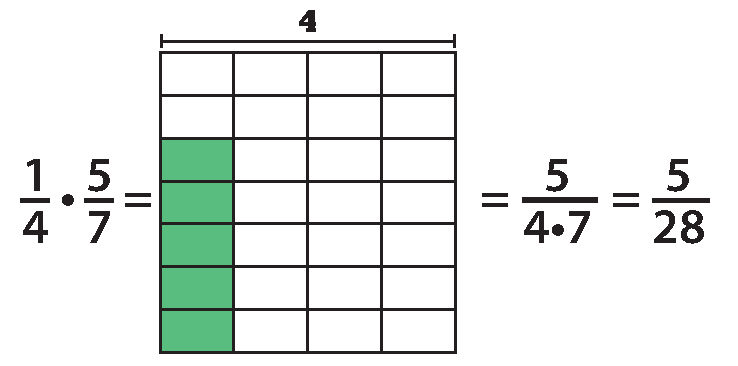
\includegraphics[scale=0.4]{pictures/Kuva3-1-4.pdf}
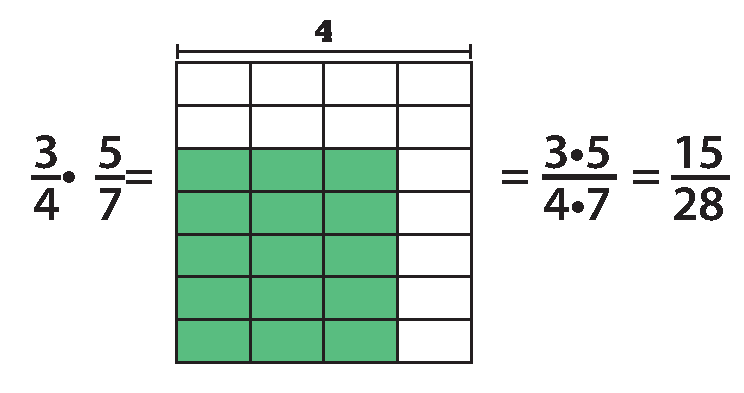
\includegraphics[scale=0.4]{pictures/Kuva3-1-5.pdf}

\begin{esimerkki}
	Luvun $5$ \termi{käänteisluku}{käänteisluku} on $\frac{1}{5}$, koska
	\[
	 5\cdot \frac{1}{5}=1.
	\]
	Vastaavasti luvun $-\frac{2}{3}$ käänteisluku on $-\frac{3}{2}$, koska
	\[
	 -\frac{2}{3}\cdot (-\frac{3}{2})=1.
	\]

\end{esimerkki}
\laatikko{
    Rationaaliluvun $a$ ($a\neq 0$) \termi{käänteisluku}{käänteisluku} on  $\frac{1}{a}$, sillä
    \[
    a\cdot \frac{1}{a} = 1.
    \]
    Vastaavasti rationaaliluvun $\frac{a}{b}$ ($a\neq 0$ ja $b\neq 0$) käänteisluku on $\frac{b}{a}$, sillä
    \[
    \frac{a}{b}\cdot \frac{b}{a} = 1.
    \]    

  %  Murtolukujen $p=\frac{a}{b}$ ja $q=\frac{c}{d}\neq 0$ \termi{osamäärä}{osamäärä} $p : q$ saadaan, kun kerrotaan luku $p$ luvun $q$ käänteisluvulla,
 %   \[
 %\frac{p}{q} = p\cdot q^{-1} = \frac{a}{b}\cdot\Big(\frac{c}{d}\Big)^{-1} = \frac{a}{b}\cdot \frac{d}{c}
 %   = \frac{ad}{bc}.
 %  \]
 }

\begin{esimerkki}
Kuinka lasketaan murtolukujen jakolasku $\frac 3 5 : \frac 2 7$? Jakolaskun määritelmän mukaan osamäärän tulisi olla sellainen luku, joka kerrottuna jakajalla antaa tulokseksi jaettavan. Jos merkitään laskun $\frac 3 5 : \frac 2 7$ vastausta kirjaimella $x$, pitää siis olla $x \cdot \frac 2 7 = \frac 3 5$.  Tätä yhtälöä kutsutaan jakolaskun $\frac 3 5 : \frac 2 7$ \termi{jakoyhtälö}{jakoyhtälöksi.}

Kerrotaan jakoyhtälön molemmat puolet luvun $\frac 2 7$ käänteisluvulla $\frac 7 2$. Koska käänteislukujen tulo on $1$, saadaan
\[
	\text{vasen puoli} = x \cdot \underbrace{\frac 2 7 \cdot \frac 7 2}_{= 1} = x \quad \text{ja} \quad \text{oikea puoli} = \frac 3 5 \cdot \frac 7 2.
\]

Kun yhtälön molemmat puolet kerrotaan samalla luvulla, ovat myös näin saadut luvut yhtä suuria. Siis on saatu
\[
	x = \frac 3 5 \cdot \frac 7 2.
\]
Koska $x$:llä merkittiin alkuperäistä jakolaskua, on nyt onnistuttu muuttamaan jakolasku kertolaskuksi:
\[
	\frac 3 5 : \frac 2 7 = \frac 3 5 \cdot \frac 7 2 = \frac{3 \cdot 7}{5 \cdot 2} = \frac{21}{10} = 2 \frac{1}{10}.
\]
Siis jakolasku laskettiin kertomalla jaettava jakajan käänteisluvulla. Näin toimitaan yleisestikin.
 \end{esimerkki}

\laatikko{
Olkoon $b \neq 0$, $c \neq 0$ ja $d \neq 0$. Murtolukujen osamäärä $\frac a b : \frac c d$ lasketaan kertomalla jaettava jakajan käänteisluvulla:
\[
	\frac a b : \frac c d = \frac a b \cdot \frac d c = \frac{ad}{bc}.
\]
}

Samannimisten murtolukujen vertailu on helppoa: jos $a > 0$, $\frac{b}{a} < \frac{c}{a}$ täsmälleen silloin kun $b < c$. Yleisten murtolukujen
vertailu voidaan tehdä siis laventamalla luvut samannimisiksi:

\laatikko{
Kahta murtolukua voidaan vertailla laventamalla ne samannimisiksi siten, että yhteinen nimittäjä on positiivinen, ja sitten vertaamalla osoittajia.
}
    
    \begin{esimerkki}
        Salamipizza jaetaan kuuteen ja tonnikalapizza neljään yhtä suureen
        siivuun. Vesa saa kaksi siivua salamipizzaa ja yhden siivun tonnikalapizzaa.
        Minttu saa kaksi siivua tonnikalapizzaa. Kumpi saa enemmän pizzaa, jos
        molemmat pizzat ovat saman kokoisia?
        
        \begin{center}        
          
\includegraphics[scale=1.0]{pictures/Kuva3-1-6-pizzat.pdf}
        \end{center}

        \textbf{Ratkaisu.}
        
        Huomataan, että $12 = 3\cdot 4 = 2\cdot 6$. Luvut kannattaa
        pizzan kokonaismäärän laskemista varten laventaa niin, että
        nimittäjänä on luku $12$.
        Vesan saama määrä pizzaa on
        \begin{align*}
           \frac{2}{6} + \frac{1}{4} &= \frac{2\cdot 2}{2\cdot 6} + \frac{3\cdot 1}{3\cdot 4} \\ 
	       							 &= \frac{4}{12}+\frac{3}{12} \\ 
	       							 &= \frac{7}{12}.
        \end{align*}
        
        Mintun saama määrä pizzaa on
        \[
            \frac{2}{4} =
            \frac{3\cdot 2}{3\cdot 4} =
            \frac{6}{12}.
        \]
        Koska $6/12 < 7/12$, Vesa saa enemmän.
    \end{esimerkki}
    
    Kaikki rationaaliluvut voidaan esittää murtolukumuodossa, mutta myös
    kokonaisluvut voidaan esittää murtolukuina asettamalla murtoluvun
    nimittäjäksi yksi. Tätä voidaan käyttää, kun lasketaan yhteen
    kokonaislukuja ja murtolukuja.
    
    \begin{esimerkki}
        Laske
        \[
            2 + \frac{1}{3}.
        \]
        
        \textbf{Ratkaisu.}
        
%        Kirjoitetaan aluksi
%        \[
%            2=\frac{2}{1}.
%        \]
		Kirjoitetaan lausekkeen kokonaisluku $2$ murtolukuna, jonka
		jälkeen voidaan murtoluvut voidaan laventaa samannimisiksi
		ja laskea yhteen:
        \begin{align*}
           2 + \frac{1}{3} &= \frac{2}{1} + \frac{1}{3}  \\ 
	       				   &= \frac{3 \cdot 2}{3 \cdot 1} + \frac{1}{3} \\ 
	       				   &= \frac{6+1}{3} \\ 
	       				   &= \frac{7}{3}.
        \end{align*}
    \end{esimerkki}
